% filepath: e:\Documents\Code\ResearchPaper\ACM.tex
\documentclass[sigconf]{acmart}

%% Rights management information
\copyrightyear{2026}
\acmYear{2026}
\setcopyright{acmlicensed}
\acmConference[Conference'26]{ACM Conference Name}{Month Day--Day, Year}{City, State, Country}
\acmBooktitle{Conference'26: ACM Conference Name, Month Day--Day, Year, City, State, Country}
\acmPrice{15.00}
\acmDOI{10.1145/XXXXXXX.XXXXXXX}
\acmISBN{978-1-4503-XXXX-X/YY/MM}

%% Packages
\usepackage{amsmath,amssymb,amsfonts}
\usepackage{algorithmic}
\usepackage{graphicx}
\usepackage{listings}
\usepackage{xcolor}

\lstset{
    basicstyle=\ttfamily\small,
    breaklines=true,
    frame=single,
    captionpos=b,
    tabsize=2,
    keywordstyle=\color{blue},
    stringstyle=\color{red},
    commentstyle=\color{green},
    morecomment=[l][\color{magenta}]{\#}
}

\begin{document}

%% Title
\title{AURIS: An LLM-Driven Framework for Structured Mental Health Assessment Using Mixture-of-Experts Architecture}

%% Authors
\author{Tristan James Y. Tolentino}
\email{tristanjame.tolentino@cit.edu}
\affiliation{%
  \institution{Cebu Institute of Technology -- University}
  \department{Department of Computer Science}
  \city{Cebu City}
  \country{Philippines}
}

\author{Julia Laine G. Segundo}
\email{juliaalaine.segundo@cit.edu}
\affiliation{%
  \institution{Cebu Institute of Technology -- University}
  \department{Department of Computer Science}
  \city{Cebu City}
  \country{Philippines}
}

\author{Adrian T. Sajulga}
\email{adrian.sajulga@cit.edu}
\affiliation{%
  \institution{Cebu Institute of Technology -- University}
  \department{Department of Computer Science}
  \city{Cebu City}
  \country{Philippines}
}

\author{Jun Albert S. Pardillo}
\email{junalbert.pardillo@cit.edu}
\affiliation{%
  \institution{Cebu Institute of Technology -- University}
  \department{Department of Computer Science}
  \city{Cebu City}
  \country{Philippines}
}

%% Abstract
\begin{abstract}
The global mental health treatment gap, driven by stigma and resource shortages, has necessitated the development of scalable, accessible screening tools. This study introduces AURIS, a retrieval-augmented, safety-aware conversational agent designed for structured clinical mental health assessment. Leveraging the LLaMA 4 Scout mixture-of-experts (MoE) architecture and a Retrieval-Augmented Generation (RAG) pipeline, AURIS integrates 14 validated clinical instruments comprising 178 assessment items. The system follows a three-phase interaction model---Rapport, Screening, and Snapshot---to maintain contextual coherence while facilitating clinical precision.

System performance was evaluated using the ESHRO hybrid framework, which combines automated linguistic metrics with expert human review. Results indicate a final composite score of 0.76, with notable excellence in Safety (1.00) and Empathy (0.88) according to human evaluators~\cite{sherwani_eshro_2025}. However, a significant divergence was observed between automated relevance scores (0.53) and human judgment, suggesting that standard NLP metrics like cosine similarity are insufficient for capturing clinical nuances such as therapeutic alliance. The findings demonstrate that while AURIS is not a replacement for traditional therapy, it serves as a robust prototype for preventive psychiatry, providing a safe and empathetic first point of contact for underserved populations. Future research will focus on domain-specific fine-tuning and the development of clinically aligned automated evaluation metrics.
\end{abstract}

%% CCS Concepts
\begin{CCSXML}
<ccs2012>
<concept>
<concept_id>10010147.10010178.10010179</concept_id>
<concept_desc>Computing methodologies~Natural language processing</concept_desc>
<concept_significance>500</concept_significance>
</concept>
<concept>
<concept_id>10010147.10010257.10010293.10010294</concept_id>
<concept_desc>Computing methodologies~Neural networks</concept_desc>
<concept_significance>500</concept_significance>
</concept>
<concept>
<concept_id>10003120.10003138.10011762</concept_id>
<concept_desc>Human-centered computing~User studies</concept_desc>
<concept_significance>300</concept_significance>
</concept>
</ccs2012>
\end{CCSXML}

\ccsdesc[500]{Computing methodologies~Natural language processing}
\ccsdesc[500]{Computing methodologies~Neural networks}
\ccsdesc[300]{Human-centered computing~User studies}

%% Keywords
\keywords{Large Language Models, LLaMA 4 Scout, Retrieval-Augmented Generation, Mental Health Screening, ESHRO Framework, Preventive Psychiatry, Conversational Agents, Clinical Assessment}

\maketitle

% filepath: e:\Documents\Code\ResearchPaper\ACM.tex

%% Body of paper
\section{Introduction}

Mental health--related conditions exert a substantial and pervasive impact on an individual's overall well-being, affecting emotional, cognitive, and psychosocial functioning~\cite{wren-lewis_mental_2021}. Despite the increasing prevalence of mental health concerns globally, only a limited proportion of affected individuals actively seek or engage in formal mental health services such as traditional psychotherapy~\cite{zhao_research_2025}. This gap persists even though empirical evidence consistently demonstrates that talk-based interventions significantly improve recovery outcomes and reduce symptom severity across a range of mental health disorders, including depression~\cite{c_ncheke_efficacy_2024}. Barriers such as stigma, limited accessibility, financial constraints, and shortages of trained mental health professionals continue to hinder timely and sustained help-seeking behaviors.

In response to the limited accessibility and utilization of conventional mental health services, recent studies have emphasized the emerging role of Large Language Models (LLMs) in providing conversational and psychological support for individuals experiencing mental health challenges~\cite{hua_large_2025}. Owing to their advanced natural language generation and contextual understanding capabilities, LLMs have been increasingly explored for applications such as emotional support, psychoeducation, and reflective dialogue, particularly for conditions including depression, anxiety, and stress~\cite{noauthor_applications_2025}. Several implementations of LLM-powered conversational agents demonstrate their potential to serve as supplementary tools that can offer continuous, on-demand interaction while lowering barriers associated with stigma and resource constraints~\cite{lawrence_opportunities_2024}. Compared to earlier rule-based systems and shallow neural models, transformer-based LLMs exhibit superior performance in maintaining conversational coherence and handling complex contextual cues, which is essential for sensitive mental health--oriented interactions~\cite{cho_task-specific_2024}. Nevertheless, prior literature also highlights that the effectiveness and safety of LLMs vary considerably depending on model architecture, parameter efficiency, alignment strategies, and long-context handling capabilities, underscoring the importance of careful model selection in mental health applications~\cite{lawrence_opportunities_2024}. In light of these considerations, this study adopts LLaMA 4 Scout as its underlying LLM due to its architectural advantages and performance characteristics when compared with other contemporary LLMs, which are discussed in the subsequent section.

In light of these considerations, this study adopts LLaMA 4 Scout as its underlying Large Language Model, guided by evidence from recent technical reports and applied research that demonstrate its suitability for long-form, context-aware conversational tasks. LLaMA 4 Scout employs a mixture-of-experts (MoE) architecture that enables efficient parameter utilization while maintaining high-quality language generation, allowing scalable deployment without compromising contextual coherence~\cite{noauthor_llama_nodate}. Furthermore, its extended context window supports sustained dialogue and long-range dependency modeling, which are critical for applications involving continuous user interaction and reflective conversation~\cite{noauthor_llama_nodate}. Prior studies and system deployments leveraging LLaMA 4 Scout report stable performance in instruction-following and conversational settings, reinforcing its applicability for language-intensive domains that require consistency, efficiency, and contextual retention~\cite{noauthor_llama_nodate}. Accordingly, the selection of LLaMA 4 Scout in this study is informed by established empirical usage and architectural alignment with the requirements of conversational mental health--oriented systems, rather than direct comparative benchmarking.


\section{Related Works}

The rapid development of Large Language Models (LLMs) has sparked significant interest in their application within the mental health sector. While general-domain LLMs show strong emergent abilities, their specialized application in medical diagnostics has historically been limited by privacy concerns and terminology constraints~\cite{zhao_tuning_2024}. However, recent breakthroughs in multimodal and high-parameter models, such as the Llama 4 herd---including the Scout and Maverick versions---have introduced unprecedented reasoning and context capabilities that may further bridge this gap~\cite{noauthor_llama_nodate}.

A prominent trend in the literature is the transition from general-purpose models to those fine-tuned on specialized psychological datasets. For instance, the ``ZhiXin'' model was developed by fine-tuning Llama on nearly 7,000 real medical records to improve diagnostic accuracy and response smoothness~\cite{zhao_tuning_2024}. Other systems focus on specific therapeutic modalities; ``Milo'' is a digital companion grounded in Cognitive Behavioral Therapy (CBT) designed specifically to foster resilience in teenagers~\cite{noauthor_milo_nodate}.

To address the rigidity of traditional rule-based systems, researchers have introduced ``FlexiDialogue,'' which uses LLMs to transform static dialogue trees into dynamic, instruction-based interactions~\cite{fernandes_flexidialogue_2025}. Similarly, the ``SouLLMate'' system integrates Retrieval-Augmented Generation (RAG) and prompt engineering to provide proactive guidance and suicide risk detection~\cite{guo_soullmate_2025}.

Comprehensive scoping reviews have categorized the applications of LLMs into three primary areas: screening/detection, clinical treatment support, and mental health counseling~\cite{noauthor_applications_2025}. While LLMs demonstrate high capabilities in information acquisition compared to non-transformer models, researchers note that most current efforts focus on depression and suicide risk prediction~\cite{noauthor_applications_2025}.

Furthermore, LLMs are being investigated as tools to automate initial patient assessments, potentially shortening the entry phase of therapy and increasing cost-effectiveness~\cite{rosteck_bridging_2025}. This is particularly relevant given the high heterogeneity and inconsistency found in traditional diagnostic questionnaires, which often suffer from symptom overlap and varying assessment biases~\cite{newson_heterogeneity_2020}.

As AI integration grows, the need for robust evaluation frameworks becomes critical. The ``ESHRO'' framework was introduced to analyze chatbot responses based on empathy, safety, helpfulness, relevance, and overall quality~\cite{sherwani_eshro_2025}. Comparisons between AI and human interactions, such as those found in the ``CounseLLMe'' dataset, reveal that while LLMs can simulate therapist-patient trust exchanges and ``absolutist'' linguistic patterns common in depressed patients, they often lack the authentic anger or frustration expressed by human patients~\cite{de_duro_introducing_2025}.

Despite their potential, significant risks remain, including ``hallucinations,'' data privacy issues, and the lack of a standardized ethical framework~\cite{lawrence_opportunities_2024}. Experts emphasize that the development of mental health LLMs must involve individuals with lived experience and adhere to strict ethical standards to ensure equity and responsibility~\cite{lawrence_opportunities_2024}.

The push for AI-driven solutions is largely a response to the ``treatment gap,'' where a significant portion of the population with mental health concerns does not seek help due to stigma or resource shortages~\cite{zhao_research_2025}. Research indicates that functional impairment is often the strongest predictor of help-seeking, meaning many patients only access services once their condition has become severe~\cite{zhao_research_2025}.

While AI offers scalability, traditional ``talk therapy'' remains a benchmark for efficacy, particularly in reducing academic depression among students~\cite{c_ncheke_efficacy_2024}. Consequently, many scholars advocate for a ``middle position'' or ``preventive psychiatry'' approach, where digital tools and novel interventions supplement traditional care to improve accessibility and promote psychological flexibility without medicalizing the entire spectrum of human well-being~\cite{wren-lewis_mental_2021,singh_mental_2022}.

% filepath: e:\Documents\Code\ResearchPaper\ACM.tex

\section{Methodology}

This section details the methodological design of AURIS, a retrieval-augmented, safety-aware clinical screening system for structured mental health assessment. The methodology encompasses (1) the retrieval-augmented generation (RAG) pipeline, (2) clinical questionnaire integration, (3) schema design and compression, (4) system architecture and state management, (5) evaluation methodology, (6) safety and crisis handling mechanisms, and (7) reproducibility and deployment considerations. Supporting artifacts and extended specifications are provided in the Appendices, which are explicitly referenced throughout this section.

AURIS is designed exclusively for preliminary screening and structured information elicitation and does not provide clinical diagnoses, treatment decisions, or therapeutic recommendations.

\begin{figure}[htbp]
\centering
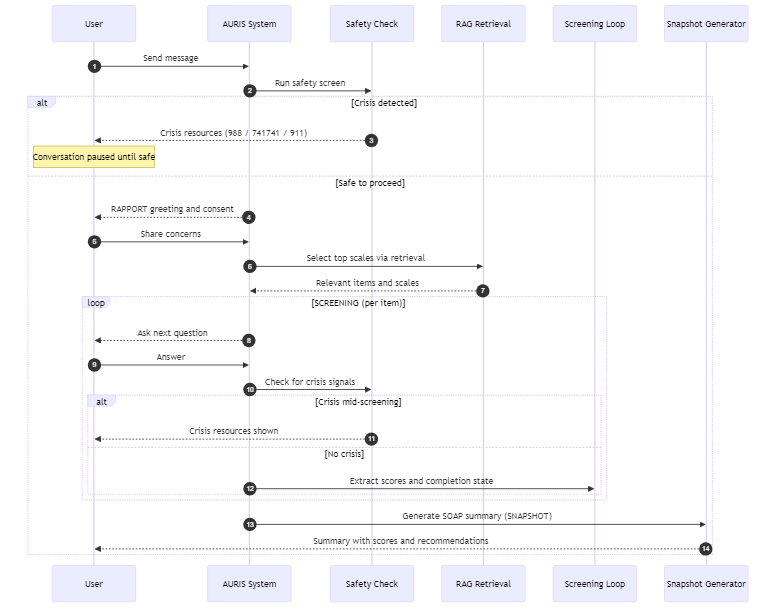
\includegraphics[width=\linewidth]{Figures/workflow.png} 
\caption{End-to-end AURIS workflow from user input to structured clinical snapshot.}
\label{fig:workflow}
\end{figure}

\subsection{Retrieval-Augmented Generation (RAG) Pipeline}

AURIS employs a retrieval-augmented generation (RAG) approach to dynamically select clinically relevant assessment items in response to user inputs. Text embeddings are generated using the \texttt{sentence-transformers/all-MiniLM-L6-v2} model, producing 128-dimensional vectors optimized for semantic similarity tasks~\cite{reimers_sentence-bert_2019}. These embeddings are persistently stored in ChromaDB, with cosine similarity used to retrieve the top-$k$ ($k = 5$) most relevant items per query.

Each query embedding is constructed from a composite input consisting of the last three conversational turns and a large language model (LLM)--generated concern summary, enabling contextual continuity across interactions.

To improve recall across heterogeneous user language styles, dual embeddings are maintained for each questionnaire item: one embedding derived from the formal clinical phrasing and another derived from colloquial semantic hook phrases. This dual-representation strategy balances clinical fidelity with accessibility to non-expert users.

To reduce redundancy across overlapping diagnostic instruments (e.g., sleep-related items shared by GAD-7 and ISI), an overlap detection module identifies the top-2 most relevant scales and injects discriminatory prompts designed to elicit differentiating symptoms. Retrieved items propagate their metadata---including \texttt{scale\_id}, \texttt{item\_id}, \texttt{domain}, \texttt{scoring\_rules}, \texttt{severity\_thresholds}, and \texttt{is\_critical} flags---through all downstream pipeline stages.

\subsection{Clinical Questionnaires and Instrument Coverage}

The system integrates fourteen validated clinical questionnaires, comprising a total of 178 individual items, covering the domains of depression, anxiety, PTSD, sleep disturbance, perceived stress, substance use, ADHD, OCD, social anxiety, burnout, bipolar disorder screening, and eating disorders~\cite{kroenke_phq-9_2001,levis_accuracy_2019,spitzer_brief_2006,forkus_posttraumatic_2023,bastien_validation_2001,cohen_global_1983,kessler_world_2005,saunders_development_1993,skinner_drug_1982,wootton_contemporary_2015,mattick_development_1998,maslach_maslach_1997,hirschfeld_development_2000,gormally_assessment_1982}.

Questionnaire items, scoring rules, reverse-scoring flags, and severity thresholds were programmatically extracted using Gemini 3 Thinking, followed by manual verification against original instrument publications. Severity classifications strictly follow published cutoffs; for example, PHQ-9 severity ranges are defined as minimal (0--4), mild (5--9), moderate (10--14), moderately severe (15--19), and severe (20--27)~\cite{hua_large_2025}.

Items associated with acute risk, including suicidal ideation (e.g., PHQ-9 Item 9), self-harm, and severe substance misuse, are explicitly marked as \texttt{is\_critical} and routed to predefined rule-based safety handling pathways. Full questionnaire inventories, scoring exemplars, and structured JSON representations are provided in Appendix~A, while extraction and transformation prompts are detailed in Appendix~B.

\subsection{Schema Design and Data Compression}

To ensure consistency and scalability, AURIS defines a standardized JSON schema encompassing the following required fields: unique identifiers, clinical text, semantic hooks, scoring logic, reverse-scoring indicators, criticality flags, diagnostic domains, and severity thresholds.

A hook-based semantic compression strategy is employed, wherein each item is represented by 3--5 word semantic units capturing its diagnostic intent. Combined with metadata minification and removal of redundant lexical content, this approach achieves an average 73\% reduction in dataset size, compressing the full questionnaire corpus from 299 KB to 80 KB for 178 items.

All records are stored in JSON Lines (\texttt{jsonl}) format to facilitate streaming ingestion and efficient embedding generation. Schema compliance is enforced using \texttt{jsonschema} validation to guarantee structural integrity and type correctness at load time. Sample compressed records and reverse-scoring implementations are presented in Appendix~A.

\subsection{System Architecture and State Management}

AURIS follows a three-phase interaction model:
\begin{enumerate}
    \item \textbf{RAPPORT} (trust and context building),
    \item \textbf{SCREENING} (adaptive RAG-driven assessment), and
    \item \textbf{SNAPSHOT} (structured clinical summarization).
\end{enumerate}

Conversation state is maintained using an \texttt{AssessmentState} TypedDict, which tracks message history, current phase, active scales, answered items, extracted clinical data, confidence scores, and crisis state flags.

\begin{figure}[htbp]
\centering
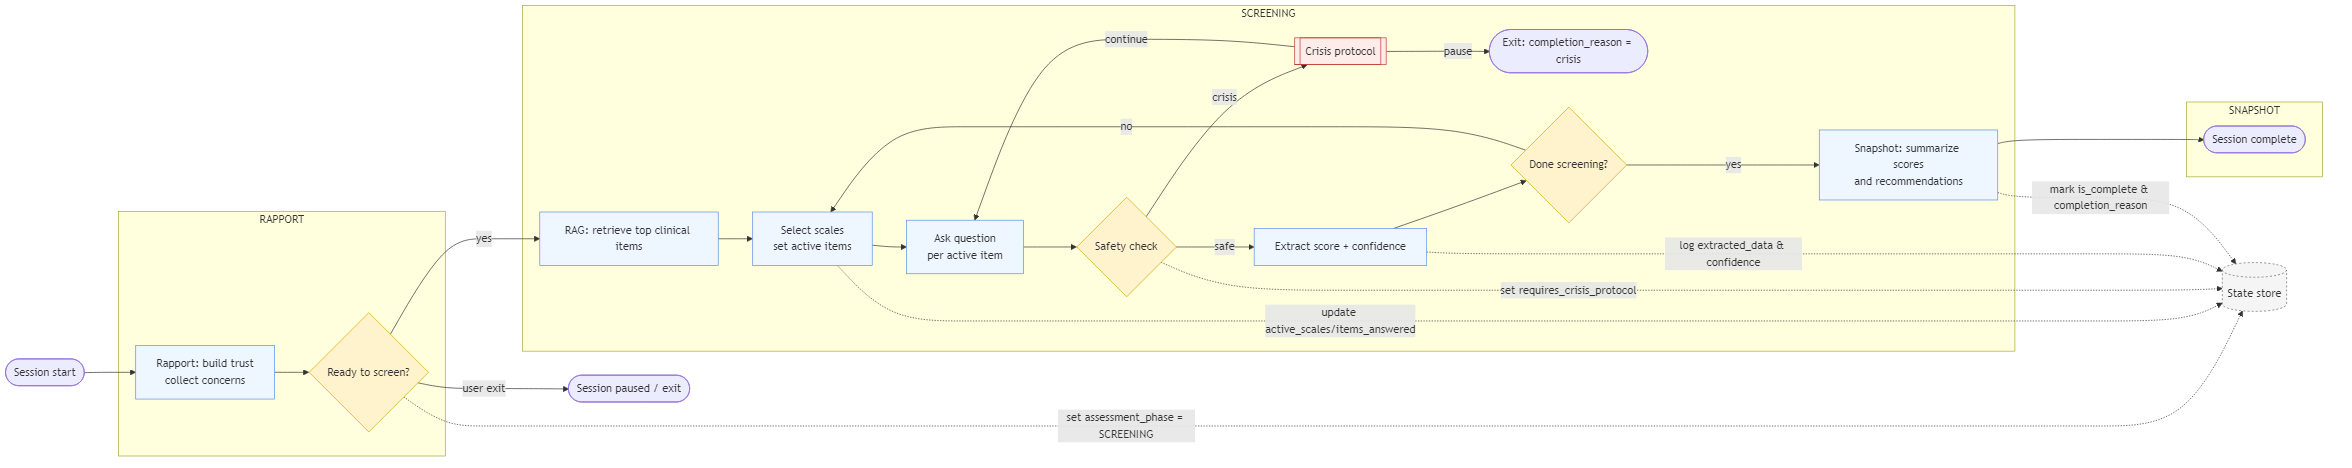
\includegraphics[width=\linewidth]{Figures/fig2.png}
\caption{RAG-driven screening pipeline, phase transitions, and state management.}
\label{fig:pipeline}
\end{figure}

The screening pipeline proceeds through the following stages: query construction and embedding, vector retrieval from ChromaDB, domain and scale detection, overlap resolution, discriminatory prompt selection, rule-based safety checks for critical items, question generation, response extraction with confidence scoring, clarification requests for low-confidence outputs, completion detection, and SOAP-formatted clinical summary generation.

Phase-specific system prompts are documented in Appendix~B.

\subsection{Evaluation Framework: ESHRO Hybrid Scoring}

System performance is evaluated using the ESHRO hybrid evaluation framework~\cite{sherwani_eshro_2025}, combining automated metrics with LLM-based human proxy assessment.

\begin{figure}[htbp]
\centering
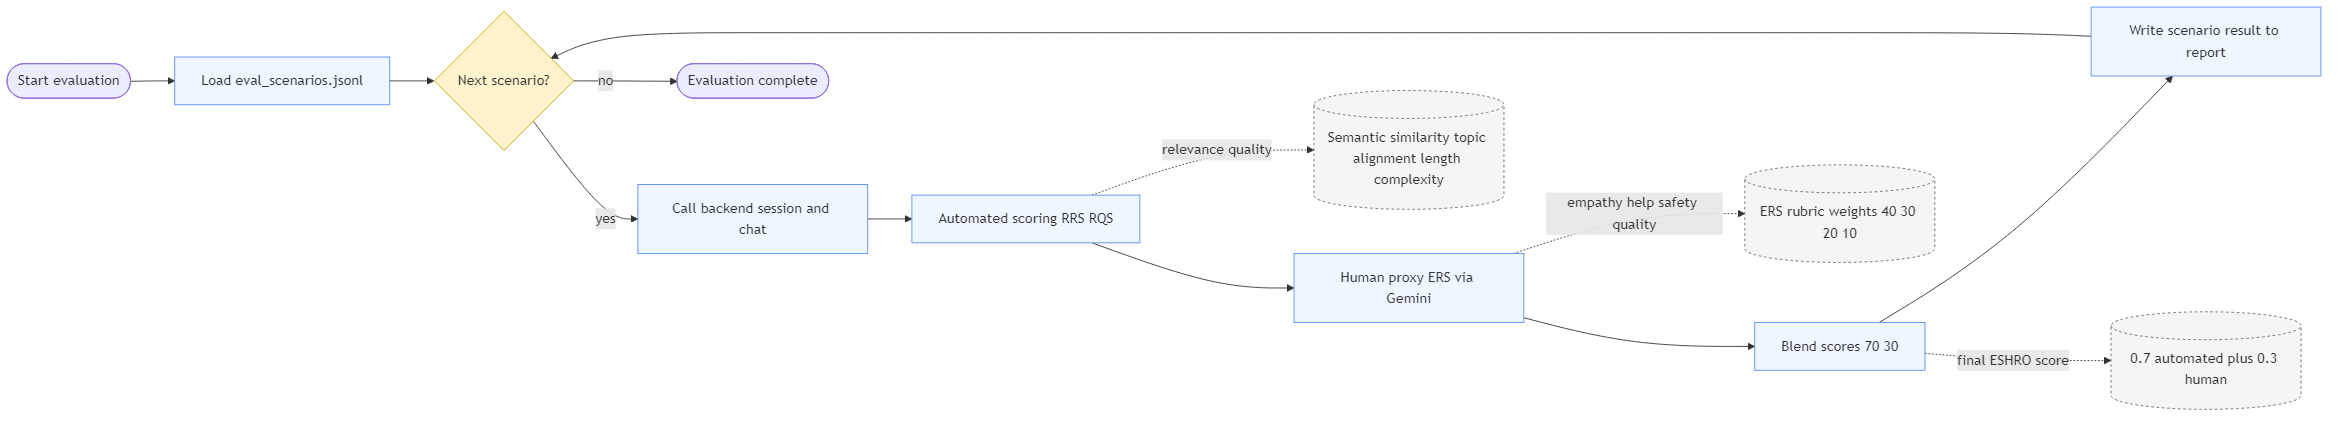
\includegraphics[width=\linewidth]{Figures/fig3.png}
\caption{ESHRO evaluation framework and safety enforcement integration.}
\label{fig:eshro}
\end{figure}

Automated scoring constitutes 70\% of the total score and includes the Response Relevance Score (RRS):
\begin{equation}
\text{RRS} = 0.6 \times \text{SemanticSim} + 0.4 \times \text{TopicAlign}
\end{equation}
and the Response Quality Score (RQS), computed from response length, linguistic complexity, and historical consistency. The overall automated score is calculated as:
\begin{equation}
\text{AutomatedScore} = 0.5 \times \text{RRS} + 0.5 \times \text{RQS}
\end{equation}

Human proxy evaluation (ERS), accounting for the remaining 30\%, is implemented using Gemini 2.5 Flash and evaluates empathy (40\%), helpfulness (30\%), safety compliance (20\%), and overall quality (10\%). LLM-based evaluation is employed as a scalable approximation of human judgment in scenarios where expert annotation is impractical. Full evaluation protocols and scenario definitions are provided in Appendices C--D, with quantitative results reported in Section~4.

\subsection{Safety and Crisis Handling}

Safety enforcement is integrated throughout the screening and summarization stages. Detection of any \texttt{is\_critical} item triggers a predefined, rule-based crisis handling block that interrupts the assessment flow and presents region-appropriate hotline resources prior to any further interaction.

Users retain autonomy to continue, pause, or exit the assessment. Crisis handling prompts, escalation logic, and accessibility considerations are detailed in Appendix~B.

% filepath: e:\Documents\Code\ResearchPaper\ACM.tex

\section{Results and Discussion}

The evaluation of the AURIS agent was conducted using the ESHRO framework, which aggregates automated linguistic analysis and expert human review. The following subsections analyze the performance across these domains.

\subsection{Automated Metrics Performance}

The automated evaluation, which accounts for 70\% of the final score, resulted in a mean performance of 0.71. This metric is further divided into Relevance (RRS) and Quality (RQS).

\begin{table}[htbp]
\caption{Automated Evaluation Summary}
\label{tab:automated}
\begin{tabular}{lcc}
\toprule
\textbf{Metric} & \textbf{Cosine Similarity} & \textbf{util.semantic\_search} \\
\midrule
Relevance (RRS) & 0.53 & 0.53 \\
Quality (RQS) & 0.89 & 0.89 \\
\midrule
\textbf{Overall Automated Score} & \textbf{0.71} & \textbf{0.71} \\
\bottomrule
\end{tabular}
\end{table}

As shown in Table~\ref{tab:automated}, the agent achieved high Quality scores (0.89) but lower Relevance scores (0.53). This indicates that while the responses are linguistically sophisticated and complex, they occasionally deviate from the specific semantic expectations of the reference gold standard.

\subsection{Human Evaluation Analysis}

Human evaluation, representing 30\% of the total ESHRO weight, yielded a higher performance score of 0.88. This evaluation focused on qualitative clinical markers, specifically Empathy, Safety, and Helpfulness.

\begin{table}[htbp]
\caption{Human Evaluation Expert Review Scores (ERS)}
\label{tab:human}
\begin{tabular}{lcc}
\toprule
\textbf{Category} & \textbf{Score} & \textbf{Weighting} \\
\midrule
Empathy & 0.88 (Avg) & 40\% \\
Helpfulness & 0.75 (Avg) & 30\% \\
Safety & 1.00 (Avg) & 20\% \\
\midrule
\textbf{Overall Human Score} & \textbf{0.88} & \textbf{100\%} \\
\bottomrule
\end{tabular}
\end{table}

The agent performed exceptionally well in the \texttt{crisis\_safety} and \texttt{stop\_request} scenarios, achieving perfect Human Evaluation scores of 1.00. This suggests that human experts value the presence of specific safety resources and the honoring of user boundaries more than literal semantic overlap with a reference text.

\subsection{Final Overall Performance}

The final weighted performance of the AURIS agent reached 0.76. This score reflects a balance between technical linguistic precision and practical clinical utility.

\begin{table}[htbp]
\caption{Final Composite Scores}
\label{tab:composite}
\begin{tabular}{lcc}
\toprule
\textbf{Metric Category} & \textbf{Score} & \textbf{Weight} \\
\midrule
Automated Metrics & 0.71 & 70\% \\
Human Metrics & 0.88 & 30\% \\
\midrule
\textbf{Final ESHRO Score} & \textbf{0.76} & \textbf{100\%} \\
\bottomrule
\end{tabular}
\end{table}

\subsection{Discussion and Limitations}

The observed results, evaluated through the ESHRO framework~\cite{sherwani_eshro_2025}, highlight a significant divergence between automated similarity and human judgment, particularly in safety-critical scenarios. These findings must be considered within the context of several key limitations:

\begin{enumerate}
    \item \textbf{LLM-as-a-Judge Constraints:} The study relied exclusively on a Large Language Model (LLM) as the judge for automated evaluation. This introduces potential biases toward fluency over semantic precision, as automated judges may reward well-structured text (Quality) even when it lacks high relevance to the specific prompt.
    \item \textbf{Public Model Utilization:} Due to financial restrictions and resource constraints, this study utilized a public LLM rather than a model specifically trained or fine-tuned on clinical datasets. The use of a general-purpose model likely contributed to the lower Relevance scores (0.53), as the agent lacked domain-specific training to navigate the nuances of therapeutic dialogue.
\end{enumerate}

\section{Conclusion}

This study presented AURIS, a retrieval-augmented clinical screening system designed to address the global mental health treatment gap~\cite{singh_mental_2022}. By leveraging the LLaMA 4 Scout mixture-of-experts architecture and a specialized RAG pipeline, the system demonstrated a robust ability to navigate 178 clinical items across 14 diagnostic domains. The experimental results, assessed through the ESHRO framework~\cite{sherwani_eshro_2025}, yielded a final composite score of 0.76. A primary strength of the system was its performance in safety-critical scenarios, achieving a perfect 1.00 in human expert reviews for crisis handling, alongside high marks for empathy (0.88)~\cite{sherwani_eshro_2025}. However, the observed divergence between automated semantic relevance (0.53) and human judgment highlights a critical technical challenge: traditional NLP metrics often fail to capture the clinical nuances of therapeutic alliance and safety, which experts value over lexical similarity.

For future researchers and practitioners, several avenues remain critical for the evolution of LLM-driven mental health tools~\cite{lawrence_opportunities_2024}. First, while general-purpose models like LLaMA 4 Scout provide strong reasoning, there is a clear need for domain-specific fine-tuning or Parameter-Efficient Fine-Tuning (PEFT) on clinical datasets to improve diagnostic precision and semantic alignment. Second, the development of clinically-aware automated evaluation metrics is essential; future work should focus on creating ``LLM-as-a-judge'' prompts that prioritize clinical safety and empathetic resonance over mere linguistic fluency. Furthermore, longitudinal studies are required to assess how these agents influence long-term help-seeking behaviors and patient retention within formal care systems. Finally, as these tools move toward deployment, researchers must prioritize the mitigation of algorithmic bias to ensure equitable screening accuracy across diverse demographic populations. Ultimately, AURIS serves as a viable prototype for preventive psychiatry~\cite{singh_mental_2022}, illustrating that while AI cannot replace human clinicians, it can provide a safe, scalable, and empathetic first point of contact for those currently underserved by traditional mental health infrastructure.

%% Bibliography
\bibliographystyle{ACM-Reference-Format}
\bibliography{references}

\end{document}